\documentclass[oneside]{llncs}
\usepackage{mydefs}
\usepackage{todonotes}
\usepackage{xspace}
\usepackage{listings}
\usepackage{pgfplots}
\usepackage{alltt}

%%%

\title{\cclj\\ Exploratory Programming for Formal Concept Analysis}
\author{Daniel Borchmann}
\institute{
  Institute of Algebra, TU Dresden\\
  \url{daniel.borchmann@mailbox.tu-dresden.de}
}

%%%

\lstdefinelanguage{Clojure}
{ alsoletter={:,-,?},
  basicstyle=\ttfamily,
  language=Lisp,
  basewidth=0.5em,
  mathescape=true,
  texcl=true,
  commentstyle=\rm,
  numbers=none
}
\lstset{language=Clojure}

\newcommand{\cclj}{\texttt{conexp-clj}\xspace}

%%%

\begin{document}

\maketitle{}

\begin{abstract}
  \cclj\ is a general purpose library tailored towards flexible and exploratory
  programming in Formal Concept Analysis.  We provide a short introduction into the design
  principles of \cclj\ and introduce some of its main features by means of various
  examples.
\end{abstract}

\section{Introduction}
\label{sec:introduction}

This is an advertisement paper for \cclj, a general purpose tool for solving certain
computational tasks in Formal Concept Analysis~\cite{ganter1999formal}.  Its main purpose
is to allow the computation of medium-sized examples which go beyond the capabilities of
manual calculation.  In particular, it is not meant to be a high-performance tool for
Formal Concept Analysis suitable for examining large amounts of data.  For this, special
programs have been developed.

\cclj is quite different from other FCA tools like ConExp~\cite{conf/kii/yevtuschenko00},
Galicia or LatticeMiner~\cite{conf/icfca/LahcenK2010}.  Those tools provide the user with
a intuitive and graphical interface which implements a fixed set of tasks.  However, the
possibilities to combine these tasks is quite limited in this setting.  On the other hand,
\cclj's main communication interface consists of a \emph{Read-Eval-Print-Loop} (REPL, also
known as a \emph{command prompt}) which allows a free combination of all the functionality
\cclj implements.  This goes so far that in some cases, \cclj is able to directly
interpret and execute simple transcriptions of mathematical algorithms, without any
further need to introduce artificial structures needed by other low-level programming
languages as C or Pascal.  This makes \cclj very suitable for \emph{exploratory
  programming} in which the user can just try out simple algorithmic ideas until she
reaches a final (or a first draft) formulation of the desired result.

The main purpose of this paper is to introduce \cclj by means of different examples, and
the structure of this paper reflects this.  In the next section we shall (briefly) discuss
the basic usage of \cclj.  Within this discussion, we shall also present some of the
details of the implementation language of \cclj, which is Clojure, a modern dialect of the
Lisp Programming Language family.  Furthermore, as Clojure emphasizes the \emph{functional
  programming} paradigm, we shall also discuss some basic principles of functional
programming.

The main part of this paper then consists of example programs in \cclj.  These examples
are not meant to be an exhaustive introduction into the main principles of \cclj.
Instead, they are meant to show the flexibility of \cclj when implementing abstract
mathematical ideas on the one hand, and, secondly, how to develop these programs starting
from only a mathematical formulation of the problem at hand.

The examples we want to discuss in this paper are the following:
\begin{enumerate}[i. ]
\item Computing the number of linear extensions of finite lattices
\item Computing the Tamari Lattice as a concept lattice
\item Computing the lattice of permutations on a given finite set
\item Computing a contextual representation of all closure systems on a finite set
\item Determining all sublattices of a given finite lattice
\end{enumerate}
Every examples introduces the necessary mathematical notions needed to understand the
problem.  Thereafter, it is shown how a \cclj could be developed that solves the problem
at hand.  Finally, we shall discuss some of the aspects and concepts used in these
programs in more detail.

We shall close this paper with a brief discussion on other features of \cclj not mentioned
in the examples discussed before.  Furthermore, we shall also discuss some of the
``non-features'' of \cclj, \ie things \cclj is not good at.  The paper then ends with a
short summary and an overview over prospective work.

\section{Basic Usage of \cclj}
\label{sec:design-princ-cclj}

In this section we shall introduce the basic usage of \cclj.  For this, we show how to
obtain and start \cclj.  After this, we discuss two design principles of \cclj and
illustrate them by means of examples.

\subsection{Obtaining and Starting \cclj}
\label{sec:obta-start-cclj}

A precompiled version of \cclj can be found on its
homepage\footnote{\url{http://github.com/exot/conexp-clj/}}.  After unpacking the file,
one can start \cclj by issuing
\begin{verbatim}
  $ conexp-clj
\end{verbatim}
on the command prompt (denoted by the ``\$'' sign; don't type that.)  After the program
has started, \cclj's prompt appears as
\begin{verbatim}
  user=> 
\end{verbatim}
From this prompt, one can use all of \cclj's functionality.  For example, if you want to
compute the sum of $2$ and $3$, just do
\begin{alltt}
  user=> (+ 2 3)
  \textit{5}
  user=>
\end{alltt}
and the program returns the result $5$ (printed in italics.)

If you want to do something more exciting like, say, creating the formal context $(\set{1,
  …, 5}, \set{1, …, 5}, ≤)$, you may say
\begin{alltt}
  user=> (make-context [1 2 3 4 5] [1 2 3 4 5] <=)
\textit{    |0 1 2 3 4 
  --+----------
  0 |x x x x x 
  1 |. x x x x 
  2 |. . x x x 
  3 |. . . x x 
  4 |. . . . x }
  
  user=> 
\end{alltt}

\subsection{Programs Should be as Simple as Possible}
\label{sec:programs-should-be}

Transforming mathematics into running programs is a difficult task, often been payed
better then the mathematical part itself.  However, most of the time a sophisticated
implementation of an algorithm is not needed, especially when one is developing an
algorithm or simply wants to have a first impression of the runtime-behavior of it.  For
these circumstances, it is a pure waste of time to develop a fine-polished implementation.
For this particular case, \cclj has been designed to allow for simple implementations of
mathematical algorithm that are very close to their mathematical formulation.  This is one
of the main reasons why the implementation language chosen for \cclj is
Clojure\footnote{\url{http://www.clojure.org}}, a dialect of the Lisp
family\footnote{``Lisp ... made me aware that software could be close to executable
  mathematics.'', L.~Peter~Deutsch}.  Since Clojure (as a Lisp) also supports paradigms of
functional programming, it is even more suitable to allow for smooth translations of
mathematics into running code.  It is the purpose of this section to describe this in (a
bit) more detail.

Let us start with a simple example first.  Suppose that you have given the set
\begin{equation*}
  \set{ x ∈ \set{ 1, …, n } \mid n \text{ odd} }.
\end{equation*}
A simple translation of this set into actual \cclj-code would be
\begin{lstlisting}
  (set-of x | x (range 1 (+ 1 n)) :when (odd? n))
\end{lstlisting}
There are a lot of things one can say about this line of code: first of all, Clojure (as a
Lisp) puts down all\footnote{almost all} its operators in \emph{prefix notation}.
Therefore, \lstinline{(+ 1 n)} is the same as $n + 1$, but only in prefix notation.  In
the same spirit, \lstinline{(range 1 (+ 1 n))} can be read as ``$\mathrm{range}(1, n +
1)$'' in standard math notation (which is also prefix in this case).  Since the
Clojure-function \lstinline{range} corresponds to an ellipsis (…) in mathematical
notation, this yields a sequence of all natural numbers from 1 (inclusive) to $n+1$
(exclusive, hence the $+1$.)  As one can easily guess, the function \lstinline{odd?}
(including the question mark) returns true if and only if its sole argument is an odd
natural number.

The special function \lstinline{set-of} then corresponds roughly to the notation ``$\set{
  … | …}$'' in mathematical writing.  If one writes $\set{x ∈ \set{ 1, …, n } \mid f(x)}$
(where $f$ denotes some arbitrary condition on $x$), the corresponding transcription is
\begin{lstlisting}
  (set-of x | x (range 1 (+ 1 n)) :when (f x))
\end{lstlisting}
(note that the element-of sign $∈$ is omitted in \cclj since it is implicitly clear from
the context.)

There are other examples where mathematical terms have a simple transcription into
\cclj-code.  For example, the formula
\begin{equation*}
  x := \sum_{i = 1}^{k}i
\end{equation*}
can be written in \cclj as
\begin{lstlisting}
  (def x (reduce + 0 (range 1 (+ 1 i))))
\end{lstlisting}
which does nothing else but creating a list from 1 to $i$ and then ``folding'' that list
by means of addition, \ie by adding the first two arguments of that list and replacing
these with the result.  This is done until the list only contains one element, which is
then returned as the result (and bound to the variable \lstinline{x}.)

Another common pattern in mathematical writing is
\begin{equation*}
  ( f(x) \mid x ∈ \set{ 1, …, n} )
\end{equation*}
which denotes a family of values under a function $f$ (and maybe also written as $\set{
  f(x) \mid x ∈ \set{ 1, …, n }}$.)  Its translation into \cclj-code can be done using the
function \lstinline{map}:
\begin{lstlisting}
  (map f (range 1 (+ 1 n)))
\end{lstlisting}
Therefore, if one wants to transform an expression of the form
\begin{equation*}
  x := \sum_{i = 1}^{k} f(i)
\end{equation*}
into \cclj-code, one could write
\begin{lstlisting}
  (def x (reduce + 1 (map f (range 1 (+ 1 n)))))
\end{lstlisting}
This always works, but maybe a bit too much.  Incidentally, \cclj provides a short
notation for this:
\begin{lstlisting}
  (def x (sum i 1 k (f i)))
\end{lstlisting}
which is as short as the original notation.  However, the reader may not have noticed but
should see that the general pattern is not that complicated as it looks like.  For
example, if one wants to compute $n!$, one can write
\begin{lstlisting}
  (reduce * 1 (range 1 (+ 1 n)))
\end{lstlisting}
since $n! = \prod_{i = 1}^n i$.

We want to note that the paradigms we have shown (as \lstinline{reduce} and
\lstinline{map}) here are inherited by the \emph{functional programming paradigm} that is
provided by Clojure.  This paradigm is very close to mathematical thinking.  However, in
some circumstances (especially when performance matters), this can be a drawback.  We
shall discuss this in a latter section.

\subsection{Support Exploratory Programming}
\label{sec:supp-expl-progr}

As already noticed, computing non-trivial medium-sized examples is the core application of
\cclj.  Having to compute these examples may occur for different reasons, but one is the
for conducting experiments and for gaining insights into unexpected
observations.\footnote{One may also call this ``playing around.''}  One example for this
may be the following: \textit{is there a correlation between the number of intents and the
  number of pseudo-intents of a formal context with $n$ attributes?}  This question arose
from experiments in~\cite{Borchmann11}, in which such a correlation has been observed
under certain circumstances.  However, to the best knowledge of the author, there has been
no further research into this direction.

To start with this experiment, it is helpful to plot for a certain amount of formal
contexts the number of their intents and the number of their pseudo-intents as a diagram.
Let us choose $n = 10$.  Then we can obtain a list of pairs of number of intents and
pseudo-intents for randomly chosen formal contexts with attribute set $\set{ 1, …, 10 }$
as follows, where we choose the number of objects randomly between 0 and 1023:
\begin{lstlisting}
  (def points (map (fn [i]
                (let [ctx (reduce-context (random-context (rand-int 1024)
                                                          10
                                                          (rand)))]
                  (list (count (intents ctx))
                        (count (pseudo-intents ctx)))))
                (range 1 1000)))
\end{lstlisting}
This will give a list of 1000 pairs of data points (from which 593 are distinct).  The
resulting diagram is shown in Figure~\ref{fig:diagram-1}.  As one can see from this
picture, the experiment shows a certain correlation between the number of intents and
pseudo-intents.

\begin{figure}[tp]
  \centering
  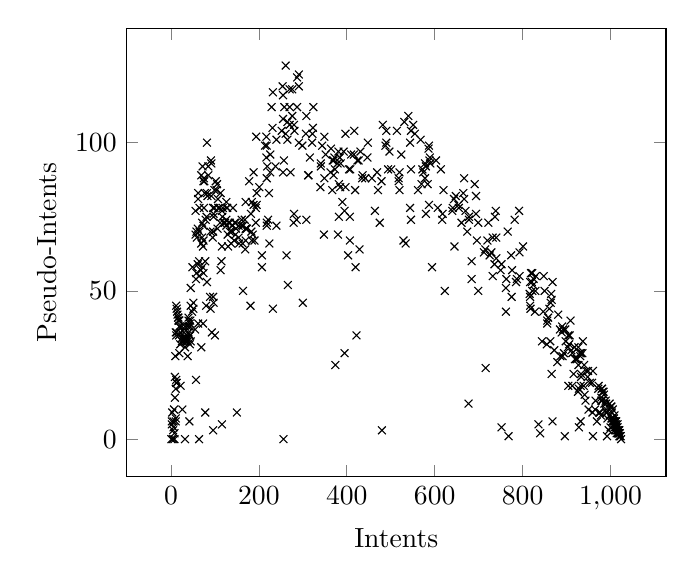
\begin{tikzpicture}
    \begin{axis}[xlabel=Intents,ylabel=Pseudo-Intents]
      \addplot[only marks, mark=x] coordinates {
        ( 972,   17) ( 982,   16) ( 993,    7) (1024,    0) (  97,   75)
        (  25,   33) ( 147,   73) (  11,   36) ( 896,    1) ( 316,   95)
        (  31,   34) ( 590,   93) ( 546,   91) ( 836,    5) ( 936,   29)
        ( 431,   97) ( 989,   13) (  30,   36) (  25,   38) (  65,   70)
        (  49,   58) (  74,   87) ( 138,   70) (1023,    1) ( 183,   70)
        (   6,    6) (  32,   38) ( 368,   94) ( 916,   22) ( 740,   68)
        (  96,   78) ( 134,   73) (  96,   70) (1021,    2) ( 145,   73)
        ( 163,   66) ( 943,   13) ( 584,   86) ( 123,   73) ( 856,   39)
        ( 524,   96) ( 286,   74) ( 372,   95) ( 858,   41) ( 750,   57)
        (  13,   44) ( 281,  104) ( 939,   18) ( 907,   35) (   1,    0)
        ( 107,   81) ( 140,   72) (   2,    5) ( 427,   94) (  12,   19)
        ( 973,   18) ( 195,   79) ( 111,   78) (  85,   92) ( 214,   99)
        (  38,   33) (1009,    4) (1013,    5) ( 164,   50) (  99,   78)
        (  22,   36) (  11,   17) ( 148,   71) ( 655,   78) (  12,   45)
        ( 417,  104) ( 981,   13) ( 116,   65) ( 715,   64) ( 381,   97)
        ( 801,   65) ( 221,   74) ( 518,   88) ( 586,   98) (   6,    4)
        ( 117,   75) ( 603,   94) ( 850,   50) ( 287,  122) ( 898,   33)
        (  97,   76) ( 766,   70) ( 578,   93) (1012,    6) ( 363,   90)
        (  14,   43) ( 231,  105) ( 217,   95) ( 270,  106) ( 891,   28)
        ( 382,   86) ( 868,    6) ( 154,   68) (  80,   45) ( 933,   21)
        ( 866,   22) (1020,    2) (  19,   40) ( 190,   67) ( 186,   69)
        ( 752,   59) (  19,   38) (1022,    1) (  33,   33) ( 897,   37)
        ( 188,   90) (  11,    7) ( 762,   43) ( 407,   75) (  55,   37)
        ( 945,   23) ( 699,   73) ( 691,   86) ( 252,  104) ( 551,  106)
        ( 546,  104) (  12,   20) ( 913,   29) ( 147,   69) ( 930,   29)
        ( 824,   52) (  11,    6) (  72,   92) (1018,    3) ( 868,   53)
        ( 287,  112) (  40,   40) ( 170,   71) ( 588,   94) ( 385,   85)
        ( 291,  119) ( 490,  100) ( 403,   62) (1011,    6) (  65,   78)
        (  78,    9) ( 722,   73) (  40,   41) (  16,   41) ( 280,   76)
        ( 120,   73) ( 861,   44) (  24,   34) (  17,   41) ( 255,  108)
        ( 540,  109) (1004,    6) (  45,   45) (  29,   33) ( 768,    1)
        ( 195,   83) (  81,   75) ( 386,   93) ( 904,   35) ( 654,   79)
        ( 992,    1) ( 240,  101) (  74,   72) ( 112,   73) ( 312,   89)
        ( 816,   49) ( 408,   91) ( 291,  100) (  28,   34) ( 141,   78)
        (  91,   94) (  20,   38) (  36,   34) ( 990,   12) ( 113,   57)
        ( 817,   53) (  57,   54) (  85,   89) (  90,   70) (  56,   69)
        ( 894,   29) (  75,   78) ( 100,   35) ( 229,  112) ( 129,   69)
        ( 678,   74) ( 822,   56) ( 819,   56) (1005,    6) ( 178,   87)
        ( 520,   90) ( 828,   43) ( 395,   29) (1017,    3) ( 370,   89)
        ( 130,   65) (  18,   35) ( 116,   77) (  64,    0) (1003,    7)
        ( 155,   66) ( 881,   42) (  96,   48) ( 501,   91) (  93,   36)
        ( 480,    3) (1009,    6) ( 382,   75) ( 182,   76) ( 980,   17)
        (  82,   83) ( 410,   96) ( 207,   62) ( 529,   67) ( 821,   53)
        ( 580,   76) ( 864,   46) ( 374,   25) ( 256,    0) ( 712,   63)
        ( 941,   15) ( 965,   10) ( 420,   58) ( 344,   99) ( 752,    4)
        ( 416,   96) ( 618,   76) (  95,   68) ( 763,   54) ( 254,  119)
        ( 139,   72) ( 321,  100) ( 990,    9) ( 261,  126) (  42,   38)
        ( 648,   82) ( 979,   14) (  10,   28) ( 308,   74) ( 469,   90)
        ( 349,  102) ( 863,   33) ( 397,  103) (1012,    4) (  68,   57)
        ( 270,  112) (  48,   43) (  72,   58) ( 341,   93) ( 696,   67)
        (  15,   42) ( 232,  117) (1018,    2) ( 667,   88) (  92,   82)
        ( 976,    9) (  73,   39) ( 380,   69) (1009,    5) ( 729,   63)
        ( 255,   90) (1016,    5) ( 848,   55) ( 488,   99) ( 822,   50)
        (  90,   44) (  13,   36) (   8,    0) ( 181,   45) ( 223,   83)
        ( 429,   64) (  75,   88) ( 933,   29) ( 924,   27) (  43,   32)
        ( 207,   58) (1008,    7) (1014,    3) ( 926,   16) ( 184,   67)
        ( 670,   77) (1010,    3) ( 226,   90) ( 986,   12) (1020,    3)
        ( 131,   73) (  74,   67) ( 762,   51) ( 534,   66) ( 998,   12)
        ( 464,   77) (  62,   81) (  44,   40) ( 978,    8) ( 644,   81)
        ( 422,   35) ( 217,  102) ( 793,   63) ( 364,   98) (  32,   31)
        (1020,    1) (  38,   38) ( 578,   88) (  45,   33) ( 447,   95)
        (  69,   89) ( 776,   57) ( 263,   62) ( 108,   78) (1002,   11)
        (  62,   39) ( 349,   88) ( 160,   72) ( 154,   72) ( 949,   23)
        ( 793,   55) ( 918,   31) ( 442,   88) ( 739,   77) ( 300,   46)
        ( 544,  100) ( 840,    2) ( 732,   55) ( 913,   18) ( 255,  116)
        (1019,    3) ( 879,   26) ( 678,   75) (1007,    6) (1014,    2)
        ( 960,   23) ( 419,   84) (  61,   59) ( 126,   74) ( 587,   99)
        ( 640,   77) ( 892,   37) (  62,   83) (1013,    6) (  35,   33)
        (1001,   11) (  33,   34) ( 218,   72) ( 134,   70) (  83,   82)
        ( 448,  100) ( 958,   19) (1011,    5) ( 518,   87) ( 340,   85)
        (1017,    2) (  74,   56) ( 280,  106) (1002,    7) ( 265,  107)
        ( 435,   88) (1005,   10) ( 424,   94) ( 580,   92) ( 514,  104)
        ( 113,   83) (   3,    9) (  18,   40) (  64,   60) ( 384,   95)
        ( 170,   67) ( 407,   67) (  17,   40) ( 740,   61) ( 661,   73)
        ( 587,   79) ( 390,   80) ( 792,   77) ( 266,   52) ( 568,  101)
        (  57,   20) (  58,   70) ( 890,   38) ( 118,   78) ( 966,   13)
        ( 979,   13) ( 620,   84) ( 531,  107) (  82,  100) ( 774,   62)
        ( 927,   31) ( 279,   73) (1019,    2) ( 299,   99) ( 218,   88)
        ( 872,   30) ( 932,   18) ( 494,   91) (1000,    4) (   2,    6)
        (1016,    4) ( 520,   84) ( 820,   56) ( 116,    5) (  73,   65)
        ( 373,   91) ( 115,   60) (  26,   10) ( 937,   33) (  71,   73)
        ( 985,   15) (1013,    4) ( 699,   50) ( 405,   91) (  59,   68)
        ( 471,   84) ( 572,   91) ( 886,   28) ( 933,   22) (  71,   68)
        (  38,   28) (  97,   46) ( 265,  101) (  45,   51) ( 998,    8)
        ( 830,   55) ( 137,   66) (  79,   74) ( 614,   91) ( 258,  112)
        (  44,   35) (  77,   83) ( 126,   80) ( 232,   44) ( 168,   74)
        (  89,   48) ( 865,   49) ( 732,   68) ( 490,  104) ( 992,    9)
        ( 272,   90) ( 322,  103) ( 623,   50) ( 555,  103) ( 397,   85)
        ( 128,   78) ( 974,    9) ( 313,   89) ( 270,  118) ( 379,   93)
        (  43,   39) ( 218,   99) ( 126,   72) (  96,    3) ( 367,   84)
        ( 589,   95) ( 948,   21) (   8,    2) ( 775,   48) (   4,    0)
        ( 127,   78) ( 716,   24) ( 906,   32) ( 785,   53) ( 641,   78)
        ( 737,   75) ( 169,   64) ( 102,   87) (  12,   35) ( 736,   59)
        (  99,   84) ( 674,   70) ( 959,    9) ( 257,   94) ( 395,   77)
        (  21,   32) (1005,    7) ( 105,   86) ( 106,   71) ( 188,   79)
        ( 927,   25) ( 341,   92) (  69,   31) ( 240,   72) (  56,   77)
        (  51,   46) ( 393,   97) ( 960,    1) (  37,   35) (   9,   14)
        ( 436,   89) ( 544,   78) ( 931,   28) ( 787,   54) ( 981,   17)
        ( 224,   66) ( 667,   81) ( 261,  103) ( 238,   92) ( 950,   10)
        ( 919,   27) ( 855,   32) (  76,   87) ( 276,  109) (  19,   29)
        (   5,    3) (   9,   21) ( 889,   36) ( 725,   62) ( 475,   73)
        ( 720,   67) (   7,   10) ( 482,  106) (  61,   71) (  42,    6)
        ( 996,    3) (1009,    8) (  82,   53) ( 969,    6) ( 193,   73)
        ( 323,  105) (  92,   93) ( 144,   67) ( 694,   82) ( 607,   78)
        ( 218,   73) (1003,    9) ( 866,   47) ( 291,  123) ( 928,    4)
        ( 574,   90) ( 308,  109) ( 370,   94) ( 694,   76) ( 184,   80)
        ( 885,   37) ( 984,   16) ( 219,   92) ( 324,  112) ( 348,   69)
        ( 825,   54) ( 677,   12) ( 909,   40) (  51,   44) ( 903,   31)
        ( 645,   65) ( 817,   48) (  40,   36) (  13,   19) (  32,    0)
        ( 990,   10) ( 193,   78) ( 164,   72) ( 665,   83) ( 904,   18)
        ( 932,    6) ( 911,   30) (  78,   60) ( 171,   71) ( 161,   74)
        ( 150,    9) ( 201,   85) ( 276,  118) ( 226,   96) ( 940,   25)
        (  22,   18) ( 497,   97) ( 194,  102) ( 104,   84) ( 170,   80)
        ( 953,   19) ( 928,   17) ( 847,   43) ( 829,   50) (  58,   56)
        ( 479,   87) (  64,   55) ( 818,   44) ( 594,   58) (  69,   66)
        ( 817,   45) ( 352,   96) ( 307,  103) ( 684,   60) ( 173,   71)
        ( 844,   33) ( 570,   86) ( 856,   40) ( 457,   88) (1008,    6)
        ( 617,   74) (  43,   38) ( 562,   84) ( 684,   54) ( 782,   74)
        ( 921,   27) (  43,   35) ( 546,   74)
      };
      \end{axis}
    \end{tikzpicture}
  \caption{Number of intents and number of pseudo-intents from randomly drawn contexts with 10 attributes}
  \label{fig:diagram-1}
\end{figure}

Without going into too much detail, let us briefly describe what this code is doing.
First of all, we map a function over the list $(1, …, 1000)$, the function getting the
current number.  This function then generates a random context via
\begin{lstlisting}
  (random-context (rand-int 1024) 10 (rand))
\end{lstlisting}
where the number of objects is uniformly chosen between 0 and 1024.  The second argument
specifies the number of attributes to be 10.  The last argument gives the ``fill-rate'' of
the formal context as the probability of an random object to have a random attribute.  The
resulting formal context is then reduced using \lstinline{reduce-context}.  From this
formal context we then compute the intents and pseudo-intents, count them and put these
two number into a list.  The resulting list \lstinline{points} therefore may look as follows:
\begin{verbatim}
  ((1024 0) (34 35) (638 64) (794 57) (1024 0) …)
\end{verbatim}

Figure~\ref{fig:diagram-1} shows some correlation between the number of intents and the
number of pseudo-intents of randomly chosen formal contexts.  However, it is not clear
whether this correlation really exists or is only an artifact of the way the experiment
has been conducted.  For example, the formal contexts we choose randomly are not uniformly
distributed and this may have some impact on the result.  There are many open questions
about the results of this experiment,
see~\cite{sage/intentsPseudointents,conf/cla/Ganter2011} for more details.

\section{Advanced Examples}
\label{sec:examples}

In the following, we want to show how to work with \cclj\ by means of some non-trivial
examples.  The main motivation for this approach of presenting the program is to present
the flexibility of \cclj's programming constructs when solving certain abstract problems
in FCA.  Of course, the selection of the examples used is subjective and not meant to show
all features of \cclj.  Furthermore, we shall not explain every detail of the presented
programs.  In particular, we are not going to give an exhaustive introduction to the main
principles of functional programming.  On the other hand, we shall try to give as much
information as possible to convey the basic meaning of the presented programs.

\subsection{Computing the Number of Linear Extensions of Finite Lattices}
\label{sec:comp-numb-line}


\subsection{Computing the Tamari Lattice as Concept Lattice}
\label{sec:comp-tamari-latt}

\subsection{The Lattice of Permutations}
\label{sec:lattice-permutations}

\subsection{The Context of All Closure Systems on a Finite Set}
\label{sec:context-all-closure}

\subsection{Determining All Sublattices}
\label{sec:determ-all-subl}

\section{Other Features of \cclj}
\label{sec:other-features-cclj}

\todo[inline]{say that \cclj has been partially integrated into sage}

\section{Non-Features of \cclj}
\label{sec:non-features-cclj}

\cclj\ has been devised as a flexible environment to try out new (and old) ideas from
Formal Concept Analysis.  Flexibility and correctness of the programs were therefore the
two main aspects when writing \cclj.\footnote{One may thing of \cclj\ as a ``pocket
  calculator for FCA.''}  However, this approach has (of course) also some drawbacks.

The first and foremost disadvantage of \cclj\ is its inherent lack of speed in certain
circumstances.\todo[inline]{continue}

no database access, no GUI

Finally, \cclj\ inherits its main data structures from its implementation language
Clojure, as well as its syntax.  This implies that the standard syntax of mathematical
languages may not always be applicable in \cclj\ programs.  The ``best'' examples for this
is the extensional notation of sets: the set $\set{ 1, 2, 3 }$ is written in \cclj\ as
\lstinline|#{1,2,3}|.  Although this notation is close to the mathematical one it is
different and may impose some difficulties on people willing to learn \cclj.  However,
it's the author's opinion that learning these little (annoying) obstacles is worth the
benefit provided by \cclj.

\section{Conclusions and Further Work}
\label{sec:concl-furth-work}

\todo[inline]{more with sage}
\todo[inline]{GUI? (if I can find a victim)}

%%%

\bibliography{fca}
\bibliographystyle{plain}

\end{document}

%%% Local Variables:
%%% mode: latex
%%% TeX-master: t
%%% ispell-local-dictionary: "american"
%%% End:

%  LocalWords:  conexp clj daniel borchmann tu dresden de Sublattices Tamari LatticeMiner
%  LocalWords:  ConExp Galicia Eval REPL
